\documentclass[a4paper, 10pt]{article}
    \usepackage[subpreambles=true]{standalone}
    \usepackage[english, american, british]{babel}
    \usepackage[utf8]{inputenc}
    \usepackage[T1]{fontenc}
    \usepackage{hyphenat}
    \hyphenation{Mathe-matik wieder-gewinnen}
    \usepackage{amsmath}
    \usepackage{import}
    \usepackage{tabularx}
    \usepackage{graphicx}
    \usepackage[margin=2cm ]{geometry}

    \title{Einführung in die Softwaretechnik 2018 \\ Sheet 04}
    \author{Maximilian Frühauf}

\begin{document}
\maketitle
\begin{enumerate}
    \item Dynamic behavior:

    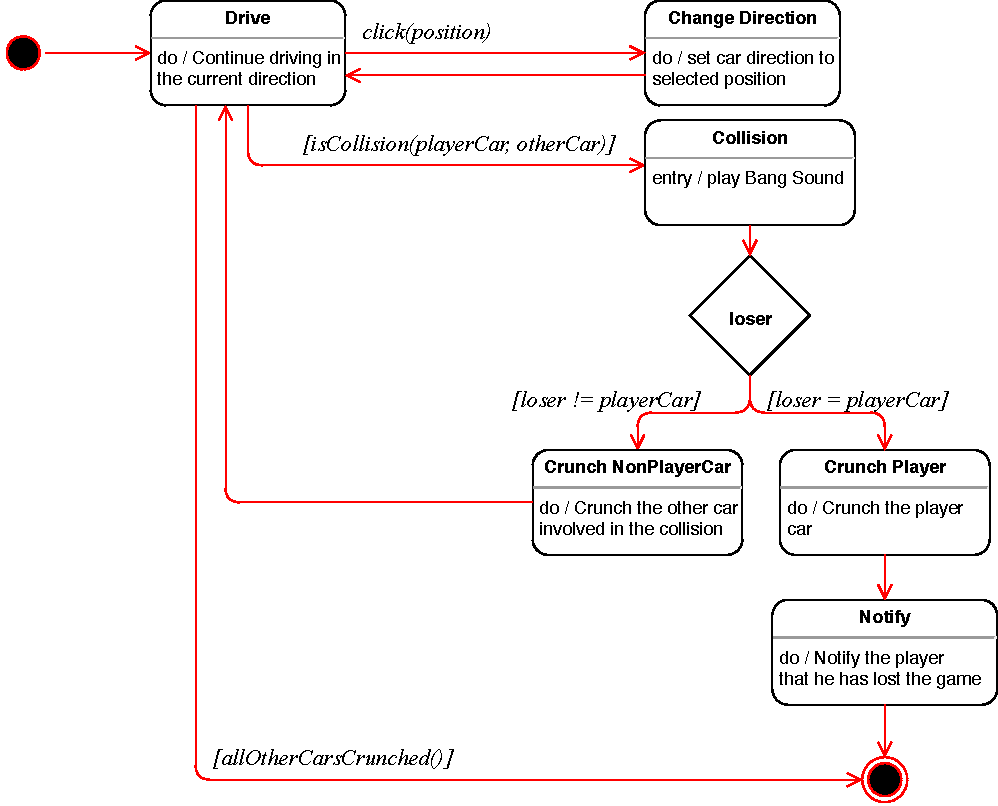
\includegraphics[width=10cm]{StateChart.pdf}

    \item Taxonomy for the car shield use case:

    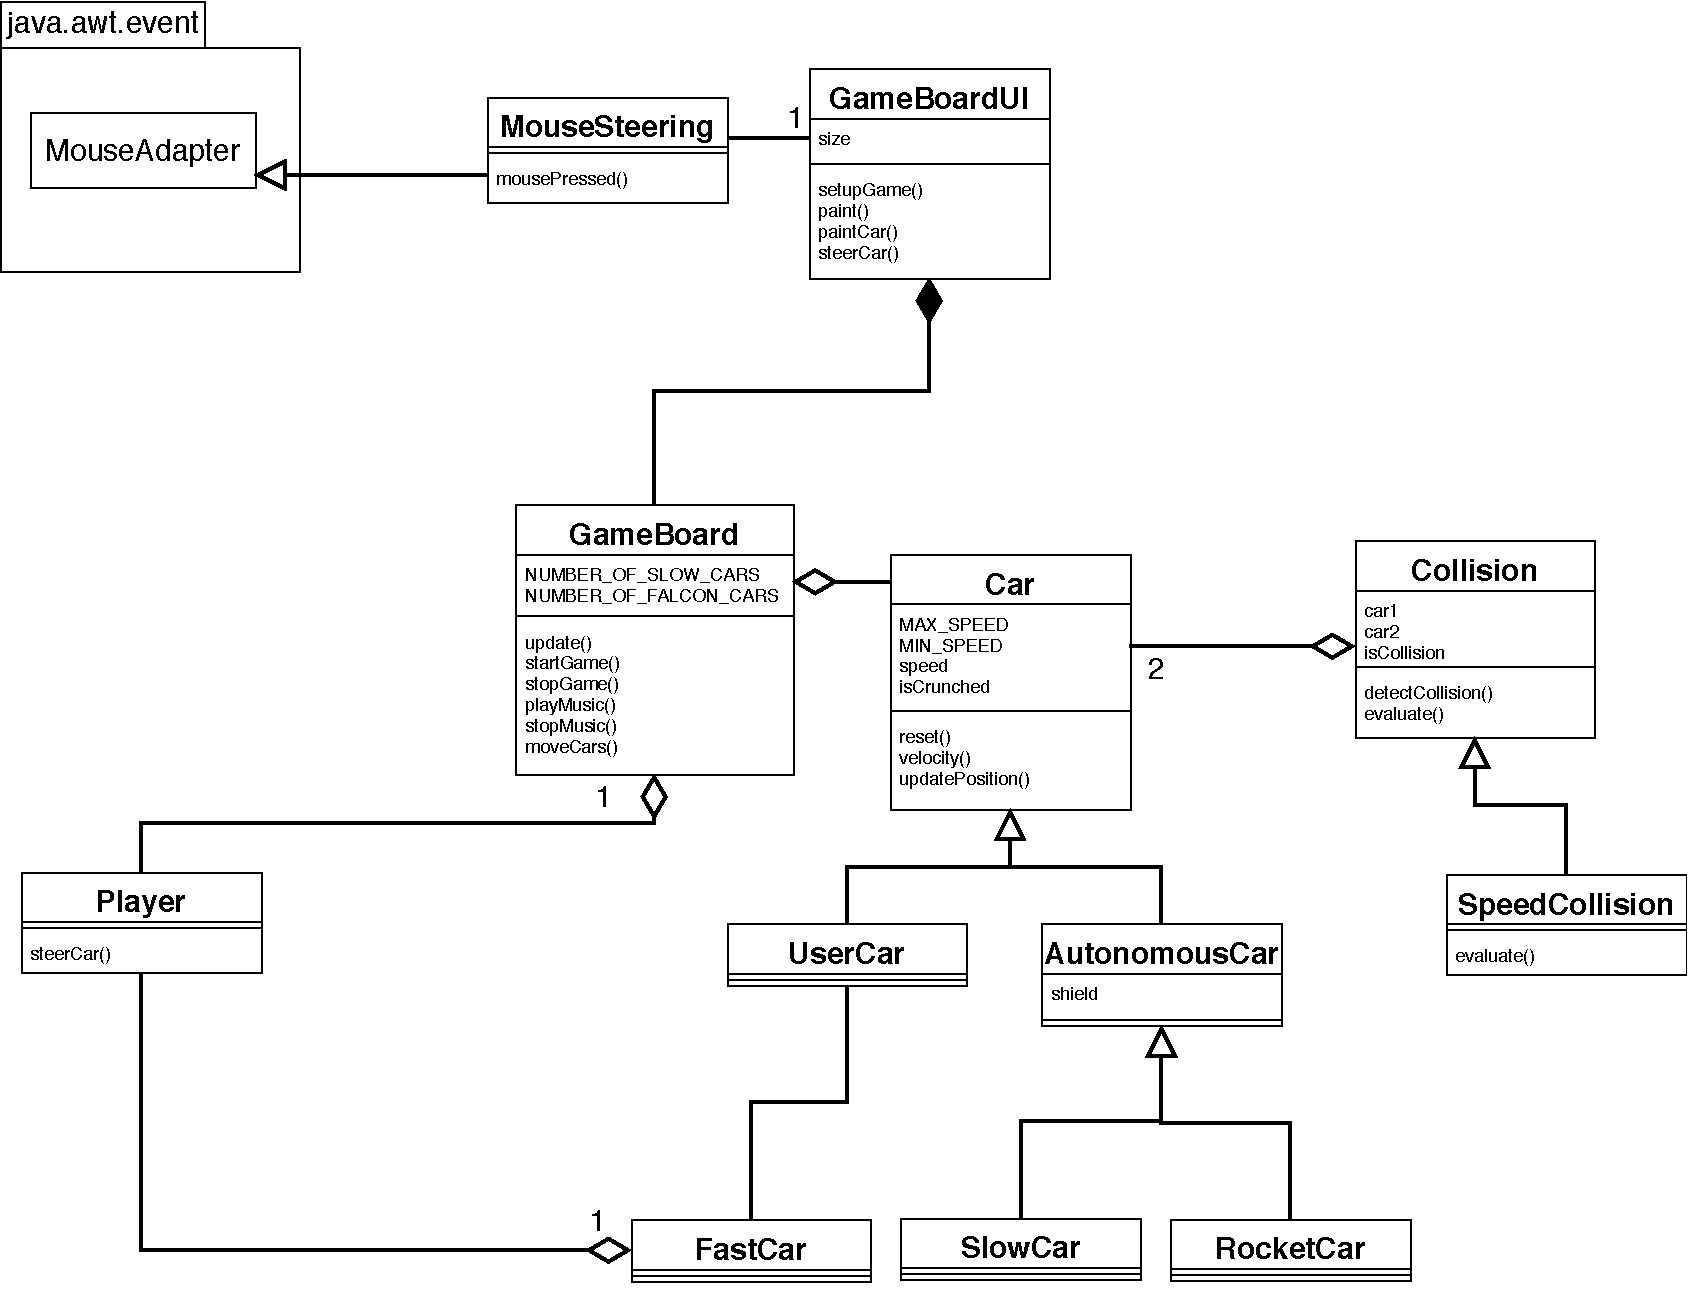
\includegraphics[width=10cm]{ClassDiagram.pdf}

    \item Win Collision activity diagram:

    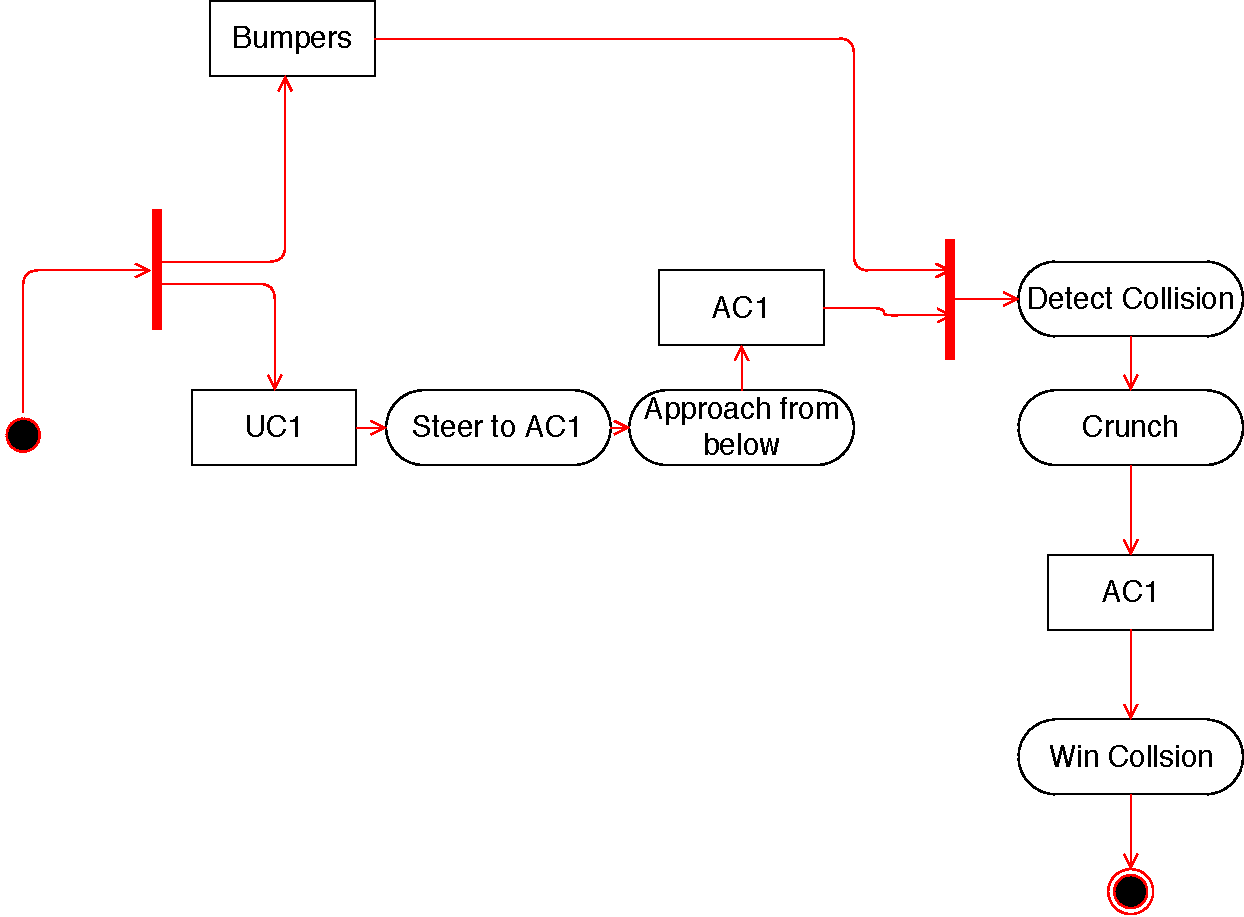
\includegraphics[width=10cm]{ActivityDiagram.pdf}

    \item Collision detection algorithm communication diagram:

    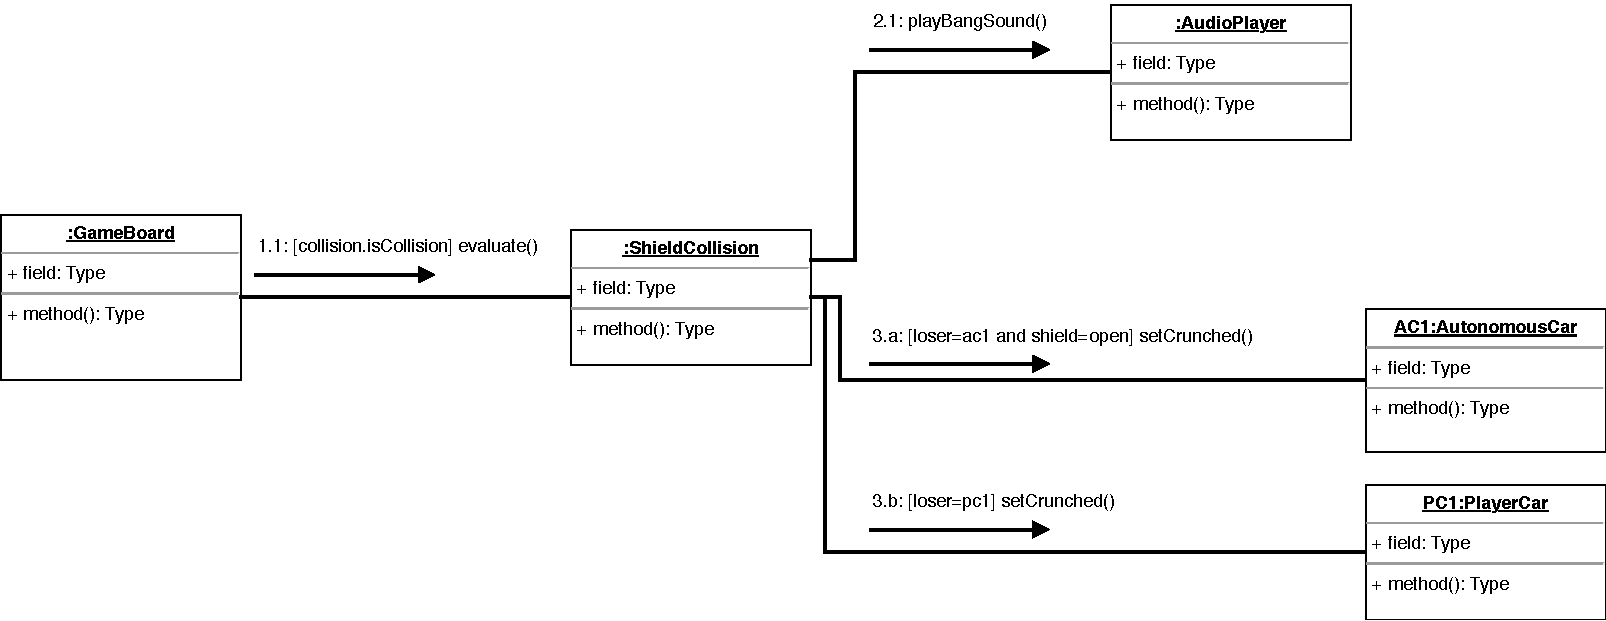
\includegraphics[width=10cm]{CommunicationDiagram.pdf}

    \item 
        Coupling measures the dependency between different subsystems inside a project.
        High coupling therefore implies that changes to one subsystem will have a large impact on 
        another subsystem.
        Low coupling on the other hand means that, a change in one subsystem does not affect others. 

        Cohesion describes the dependency among two classes. 
        Therefore high cohesion describes a subsystem where the classes perform similar tasks and 
        are related to each other in many associations.
        Low cohesion is the inverse of the above. A subsystem with many classes that handle very different
        tasks and have few to no associations with each other.

        These terms can be used to describe a good system design, as a good system should have 
        high cohesion and low coupling between the different submodules.

        // TODO: example
\end{enumerate}
\end{document}